% 问题二候选正文；条件模型及 E1/E2 推导待独立科学评审。
% 已接入 paper/main.tex 供协作排版审阅，不代表组合模型已通过科学验收。
\section{跨维度数据融合与广义标度律}
\label{sec:q2}

\subsection{问题分析与数据口径}

题目要求将参数规模、训练数据量、数据质量和领域配比纳入统一的损失回归分析，并且讨论资源的边际收益及领域之间的替代与互补关系。难点在于附件 A 与 B来源于不同的训练实验：A 包含领域配比和第一问得到的质量评价分数，B1 包含规模与训练量，B6/B7 给出质量扰动，但是A、B缺少唯一的id号等将四个量统一在一个样本集中，实际数据条件难以建立同时观测四类输入的分析模型。因此先分别估计能够由数据支持的分项，再明确建立不同来源数据之间的对应关系，并说明关联规则与基本假设；分项验证单个模型、并且组装成组合模型进一步验证组合模型的有效性。

\subsection{分项估计与条件组合模型}
记 $N$ 为十亿参数数，$D$ 为十亿训练 token 数，$L$ 为损失；$\boldsymbol p\in\Delta_{17}$ 为 17 个领域的训练占比，$\Delta_{17}=\{\boldsymbol p\geq\boldsymbol 0:\boldsymbol 1^\top\boldsymbol p=1\}$。第一问给出的领域质量分数组成 $\boldsymbol q$，定义基于附件A构建的数据质量代理指标 $Q_A=\boldsymbol q^\top\boldsymbol p$。默认采用 TOPSIS 分数轴，同时以 soft 分数轴检查敏感性。这里 $Q_A$ 是配比 (\boldsymbol p) 的函数，其变化与配比调整相联系，相关结果反映的是给定配比变化路径下的质量效应。

以题设幂律形式为规模基线，使用 B1 中相同的小规模实验数据拟合两个模型，并在预先留出的大规模实验数据上比较预测误差，以检验所提模型相对于对数线性基准模型的外推能力。规模分项写为
\begin{equation}
L_{\mathrm{scale}}(N,D)=E+AN^{-\alpha}+BD^{-\beta},\qquad A,B,\alpha,\beta>0.
\label{eq:q2-scale}
\end{equation}
在 B1 上拟合得到 $E=1.689798$、$A=0.353980$、$B=1.240306$、$\alpha=0.339977$、$\beta=0.279878$。拟合支持范围为 $N\in[0.070542,11.965825]$、$D\in[0.134,299.893]$，单位均为十亿；两个区间分别表征各变量的边际取值范围，联合训练观测则对应数据集中实际出现的变量组合。

将 A 质量代理映射到 B7 质量坐标。仅用 A4/A5 的 512 个训练配方确定两条质量轴各自的 $q_{\min},q_{\max}$，令
\begin{equation}
T(Q_A)=\operatorname{clip}\!\left(0.1+0.9\frac{Q_A-q_{\min}}{q_{\max}-q_{\min}},\,0.1,\,1\right),
\qquad Q_{A0}=\boldsymbol q^\top\boldsymbol p_0,
\label{eq:q2-map}
\end{equation}
其中 $\boldsymbol p_0$ 为上述训练配方均值；此映射是把两套评分范围接合的假设。为避免将 $Q_A$ 和完整配比中同一方向重复计入，先在 A4/A5 训练集计算
\begin{equation}
\boldsymbol v=\frac{\sum_i(Q_{Ai}-Q_{A0})(\boldsymbol p_i-\boldsymbol p_0)}
{\sum_i(Q_{Ai}-Q_{A0})^2},\qquad
\boldsymbol r(\boldsymbol p)=\boldsymbol p-\boldsymbol p_0-\boldsymbol v(Q_A-Q_{A0}).
\label{eq:q2-residual}
\end{equation}
在训练样本上，$\boldsymbol r$ 与 $Q_A$ 的样本协方差为零；该线性残差化刻画了二者在线性相关层面的正交关系，其统计解释限于线性相关结构，因果效应的识别则需要额外的识别条件与研究设计。令 $\widehat{\boldsymbol w}$ 为 A4/A5 上以 13 域平均 Loss 为目标、对 17 个中心化配比进行 Ridge 回归所得载荷，惩罚系数为 $10^{-5}$。质量斜率 $c=-0.361995$ 来自 B7；跨来源迁移强度 $\lambda_Q,\lambda_p\in\{0,0.5,1\}$ 为预设情景参数。组合式为
\begin{equation}
\boxed{\begin{aligned}
\widehat L_B(N,D,Q_A,\boldsymbol p)
={}&1.689798+0.353980N^{-0.339977}\\
&+1.240306D^{-0.279878}-0.361995\lambda_Q[T(Q_A)-T(Q_{A0})]\\
&+\lambda_p\widehat{\boldsymbol w}^{\top}\boldsymbol r(\boldsymbol p).
\end{aligned}}
\label{eq:q2-joint}
\end{equation}

\subsection{分层检验与迁移结果}

留一规模检验在 B1 的 8 折共汇总 1176 行。幂律的 MAE/RMSE 为 $0.000108/0.000151$，对数线性原型为 $0.090739/0.123077$，所以选式~\eqref{eq:q2-scale} 为该文件的规模项。图~\ref{fig:q2-b1} 分别展示了各轮验证中，模型在留出数据上的预测误差；点之间不连线，因为规模折彼此独立。B1 的近乎精确拟合反映数据特征采用幂律形式拟合较为精确。采用 B1 数据得确定确定的计算模型预测 B2、B4、B5，MAE 分别升至 $1.178442$、$0.227263$、$0.170722$，显示绝对 Loss 存在来源差异。

\begin{figure}[htbp]
\centering
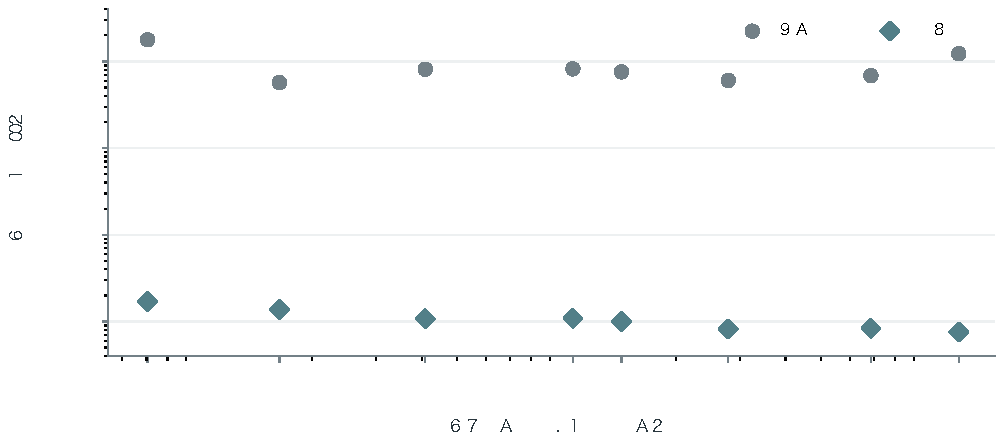
\includegraphics[width=0.88\linewidth]{figures/q2-scaling-law/Fig01_B1_leave_size.pdf}
\caption{B1 留一参数规模验证}
\label{fig:q2-b1}
\end{figure}

质量项验证 B1 规模参数，并让“无 $Q$”基线与“加 $Q$”模型使用相同的来源截距。B7 按 $(N,D)$ 组合分组留出时，MAE 从 $0.101965$ 降至 $0.057322$；留出完整质量水平时，从 $0.110407$ 降至 $0.057046$；用 B6 训练并预测 B7 中不重叠的新增 90 行时，从 $0.057491$ 降至 $0.044603$（图~\ref{fig:q2-quality}）。这些比较支持当前半合成数据设定下的质量效应（展开解释）；由于分组验证结果同时参与了质量项线性形式的确定，因此其主要作用是为模型选择提供验证依据；最终模型的独立测试性能则需由模型选择过程之外的独立测试数据进行评价。

\begin{figure}[htbp]
\centering
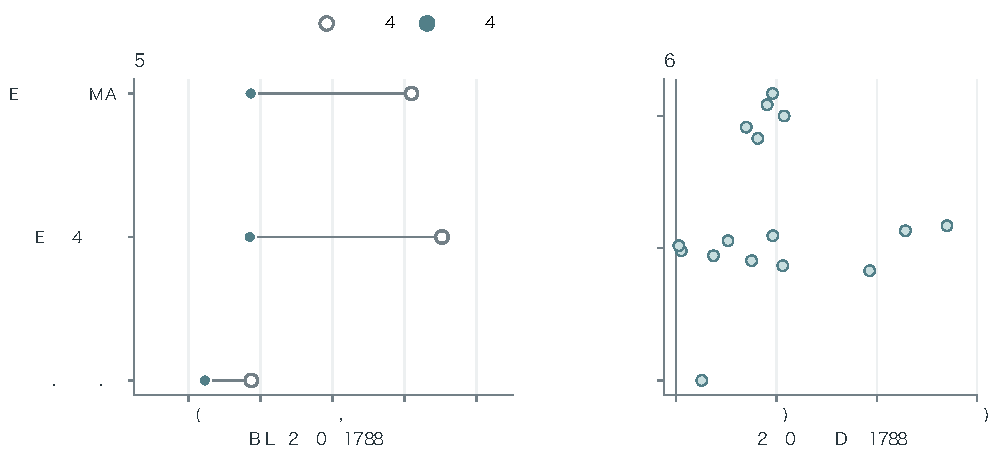
\includegraphics[width=0.9\linewidth]{figures/q2-scaling-law/Fig02_quality_increment.pdf}
\caption{引入 $Q$ 后的误差变化}
\label{fig:q2-quality}
\end{figure}

针对不同数据来源之间的系统性差异，后续需开展嵌套留出验证：外层留出 B2 的完整训练轨迹，内层选择校准形式；A 按不同配方进行外层留出与内层选择。表~\ref{tab:q2-transfer} 记录外层汇总值，图~\ref{fig:q2-transfer} 显示逐折误差。B2 校准后虽优于均值基线，残差与 $\log D$ 的 Spearman 相关仍约为 $0.9961$--$0.9979$，表明截距校正没有消除曲线形状偏差。在附件A的60M实验中，利用目标规模的部分已知损失进行校准后，配比预测误差低于均值基线；但在1B实验中，经内层验证选出的预测方法仍未优于均值基线。现有结果支持在各参数规模下分别估计和验证相应的配比迁移关系，同一套配比迁移系数的跨规模适用性则需进一步通过独立数据加以验证。

\begin{table}[htbp]
\centering
\caption{来源与配比迁移的外层留出 MAE}
\label{tab:q2-transfer}
\begin{tabular}{lrrr}
\toprule
目标 & 未校准 & 嵌套选择 & 简单均值基线 \\
\midrule
B2 规模轨迹 & 1.178442 & 0.266023 & 0.372331 \\
A 60M 配方 & 1.508086 & 0.146142 & 0.167310 \\
A 1B 配方 & 3.190256 & 0.040878 & 0.039563 \\
\bottomrule
\end{tabular}
\end{table}

A6/A7 的 256 行同规模配比检验中，完整配比模型的 MAE 为 $0.180679$，训练均值基线为 $0.225599$。质量残差配比模型为 $0.184309$；把 A 质量分量替换为 B7 质量斜率并保留 A 训练截距后为 $0.180795$。该结果适用于保持其余模型设定不变、仅调整附件 A 中相应建模组件的比较情景。跨规模时，扣除各测试集均值的配比形状 RMSE 在 60M 为 $0.1943$，低于常数模型的 $0.2189$；到 1B 时为 $0.1615$，高于常数模型的 $0.0519$（图~\ref{fig:q2-mixture}）。该中心化误差基于目标测试集的真实损失均值进行校准，主要用于评价配比响应的相对变化；实际预测误差则应在无需目标规模真实损失校准的条件下单独评估。
\begin{figure}[htbp]
\centering
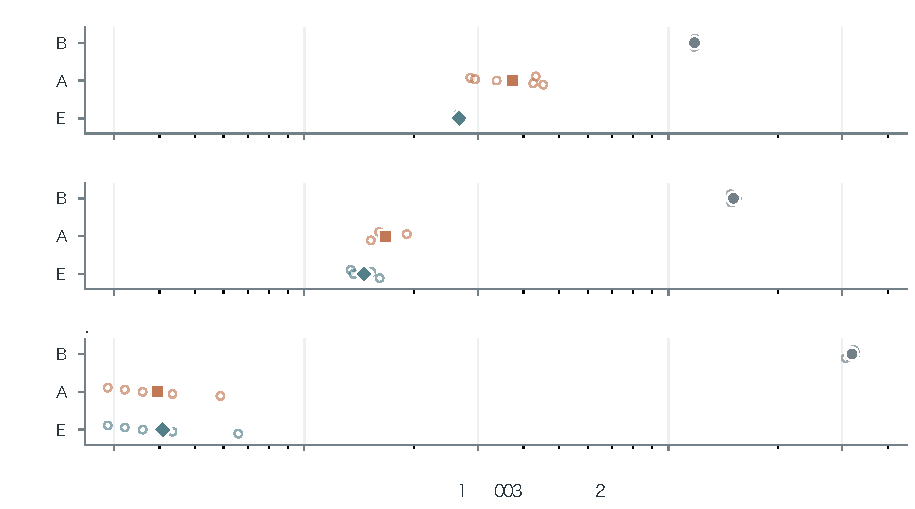
\includegraphics[width=0.9\linewidth]{figures/q2-scaling-law/Fig03_transfer_calibration.pdf}
\caption{迁移到 B2、A 60M 和 A 1B 时的外层误差}
\label{fig:q2-transfer}
\end{figure}

\begin{figure}[htbp]
\centering
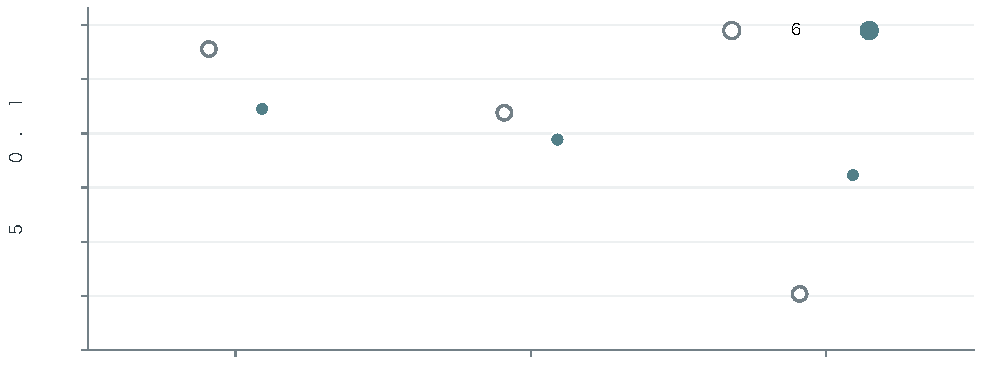
\includegraphics[width=0.86\linewidth]{figures/q2-scaling-law/Fig04_mixture_scale.pdf}
\caption{附件A 不同参数规模的配比响应形状}
\label{fig:q2-mixture}
\end{figure}


\subsection{边际收益、弹性与等效规模条件}

将质量和配比固定，定义单位资源带来的正向 Loss 改善率 $U_N=-\partial\widehat L_B/\partial N$、$U_D=-\partial\widehat L_B/\partial D$。于是
\begin{equation}
\begin{aligned}
U_N&=\alpha AN^{-\alpha-1}, & U_D&=\beta BD^{-\beta-1},\\
\frac{\partial^2\widehat L_B}{\partial N^2}&=\alpha(\alpha+1)AN^{-\alpha-2}>0,\\
\frac{\partial^2\widehat L_B}{\partial D^2}&=\beta(\beta+1)BD^{-\beta-2}>0.
\end{aligned}
\label{eq:q2-marginal}
\end{equation}
正的二阶导数表示增加资源后损失下降的幅度递减。对\emph{完整} Loss 的弹性为
\begin{equation}
\varepsilon_N=-\frac{\alpha AN^{-\alpha}}{\widehat L_B},\qquad
\varepsilon_D=-\frac{\beta BD^{-\beta}}{\widehat L_B}.
\label{eq:q2-elasticity}
\end{equation}
在 $N=1$、$D=100$、$\boldsymbol p=\boldsymbol p_0$ 和 $\lambda_Q=\lambda_p=1$ 的计算锚点，$\widehat L_B=2.385578$，$U_N=0.120345$、$U_D=0.000957$，$\varepsilon_N=-0.050447$、$\varepsilon_D=-0.040100$。$U_N$ 和 $U_D$ 的单位分别是每十亿参数和每十亿 token 的局部 Loss 变化，不能凭数值大小比较资金效率；两种资源翻倍后，各自的单位边际收益变为原来的 $39.50\%$ 和 $41.18\%$。上述参考情景下的损失、边际收益及弹性均为模型计算结果，主要用于刻画不同输入组合下的模型响应特征；四类输入组合模型的独立验证则需依据新增真实训练实验的观测结果开展。

在质量映射的内部区间，若沿保持 $\boldsymbol r$ 不变的条件路径改变 $Q_A$，则
\begin{equation}
\left.\frac{\partial\widehat L_B}{\partial Q_A}\right|_{\boldsymbol r}
=c\lambda_Q\frac{0.9}{q_{\max}-q_{\min}},\qquad c=-0.361995;
\label{eq:q2-quality-derivative}
\end{equation}
截断区该形式导数为零，边界处只定义单侧导数。TOPSIS 和 soft 轴在 $\lambda_Q=1$ 时的内区斜率分别为 $-2.605474$ 和 $-0.675302$，两轴的分数单位不同，斜率绝对值不能直接比较。质量弹性还依赖分数原点，所以仅在同一评分定义下解释。

题目所问的“质量提高 $0.1$ 等效增加多少参数”需考虑先指定质量单位。设映射后的 B 侧质量坐标 $z=T(Q_A)$ 增加 $\Delta z=0.1$，假定质量提高的全过程均位于质量映射的未截断线性区间内，同时保持训练 token 总量 \(D\) 以及剔除质量线性关联后的配比残差 \(\boldsymbol r\) 不变。令增加参数后的规模收益等于质量收益，则
\begin{equation}
A\{N_{\mathrm{eq}}^{-\alpha}-N^{-\alpha}\}=c\lambda_Q\Delta z,
\qquad
N_{\mathrm{eq}}=\left(N^{-\alpha}+\frac{c\lambda_Q\Delta z}{A}\right)^{-1/\alpha},
\label{eq:q2-equivalent}
\end{equation}
前提是括号内严格为正，且 $N_{\mathrm{eq}}$ 位于经验支持范围。以 $N=1$、$\lambda_Q=1$ 代入，得到 $N_{\mathrm{eq}}\approx1.373$，即模型中映射质量轴增加 $0.1$ 的 Loss 改善，约等于参数从 10 亿增至 13.73 亿。若题目中的 $0.1$ 指 A 的原始评分 $Q_A$，应以 $\Delta z=T(Q_A+0.1)-T(Q_A)$ 代入，该数值由计算起点与截断范围共同决定，因此应根据当前设定重新计算相应结果，13.73 亿仅对应原有设定下的计算值。由于质量评分 \(Q_A\) 由固定的领域质量分数与训练配比共同确定，保持配比残差不变并调整 \(Q_A\) 对应于指定路径下的模型计算，其结果主要用于刻画该路径下的模型响应；真实语料质量改善的实际效果则需通过独立训练实验进行验证。上述等效关系比较预测损失的变化，未考虑实现不同方案所需的费用。由于缺少参数扩容与质量提升的成本数据，现阶段尚不能判断哪种方案在经济上更优。

\subsection{领域替代、互补与情景敏感性}

固定总训练量，令 $\boldsymbol p(\delta)=\boldsymbol p_0+\delta(\boldsymbol e_i-\boldsymbol e_j)$ 表示从领域 $j$ 向 $i$ 转移配比 $\delta$。在质量映射内部，冻结模型给出
\begin{equation}
\boldsymbol g=\nabla_{\boldsymbol p}\widehat L_B
=c\lambda_Q\frac{0.9}{q_{\max}-q_{\min}}\boldsymbol q
+\lambda_p\{\widehat{\boldsymbol w}-(\widehat{\boldsymbol w}^{\top}\boldsymbol v)\boldsymbol q\},
\qquad \frac{\mathrm d\widehat L_B}{\mathrm d\delta}=g_i-g_j.
\label{eq:q2-substitution}
\end{equation}
$\delta=0.01$ 表示 1 个百分点；$g_i-g_j<0$ 表示模型预测转移后 Loss 降低。为限制推论范围，对 272 个有向领域对求解训练配方凸包内的最大转移量，并以最优边界的 $99\%$ 作安全上限。0.1、0.5、1、2、5 个百分点分别有 272、256、224、165、117 个方向通过该上限；安全上限的中位数为 4.068 个百分点。这里的特征支持单指调整后的配方能够表示为已有训练配方的非负加权平均，且权重之和为1；该配方属于模型推演得到的候选方案，其实际训练效果需通过相应的真实训练实验进一步验证。

在 $\lambda_Q=\lambda_p=1$ 时，136 个无序领域对中有 12 对在 TOPSIS 与 soft 质量轴下预测方向相反。扩大到 $\lambda_Q,\lambda_p\in\{0,0.5,1\}$ 的非全零情景后，107 对出现正负翻转；这包含关闭某一分项的压力情景。因而不依据式~\eqref{eq:q2-substitution} 排列全局领域优劣。

为检查模型能否刻画互补，取共同供给领域 $k$，使 $\boldsymbol p_{10}=\boldsymbol p_0+h(\boldsymbol e_i-\boldsymbol e_k)$、$\boldsymbol p_{01}=\boldsymbol p_0+h(\boldsymbol e_j-\boldsymbol e_k)$，并令 $\boldsymbol p_{11}=\boldsymbol p_0+h(\boldsymbol e_i+\boldsymbol e_j-2\boldsymbol e_k)$。定义四角差
\begin{equation}
I_{ij\mid k}=\widehat L_B(\boldsymbol p_{11})-\widehat L_B(\boldsymbol p_{10})
-\widehat L_B(\boldsymbol p_{01})+\widehat L_B(\boldsymbol p_0).
\label{eq:q2-interaction}
\end{equation}
在 A4 配方凸包内的 2040 个四角设计、两条质量轴共 4080 次条件计算中，$\max|I_{ij\mid k}|=8.88\times10^{-16}$ Loss，处于数值零水平。原因是映射内部式~\eqref{eq:q2-joint} 关于 $\boldsymbol p$ 为仿射函数；零交互由当前模型结构设定所决定，其含义限于模型假设下的交互形式。当凸包外的候选配方使四角设计跨越质量映射的截断边界时，截断规则本身可能导致非零四角差。这种非加性由当前模型结构产生，反映的是模型设定下的响应特征。

由于式~\eqref{eq:q2-joint} 中 $N,D$ 与质量、配比项可加分离，固定配比下 $U_N,U_D$ 不随质量情景而改变；质量与配比影响式~\eqref{eq:q2-elasticity} 的分母，并影响领域转移方向。质量因素对最优 \(N/D\) 的影响需要结合质量提升与资源投入之间的成本耦合关系进行分析。若将来取得相同 $N,D$、统一评价集下不同质量与四角配方的真实重复训练，可以再估计跨块交互和实际互补强度。

\subsection{结论与适用范围}

图~\ref{fig:q2-b8} 显示 B8 的组内质量方向与 B6/B7 不完全一致，因此 B8 未参与质量斜率估计。图~\ref{fig:q2-range} 将 B1 的拟合支持范围与 B9/B10 的参数范围并列展示，其中超出 B1 支持范围的参数规模延伸用于描述模型的外推情景，其预测精度需通过相应规模的独立观测数据进一步验证。

\begin{figure}[htbp]
\centering
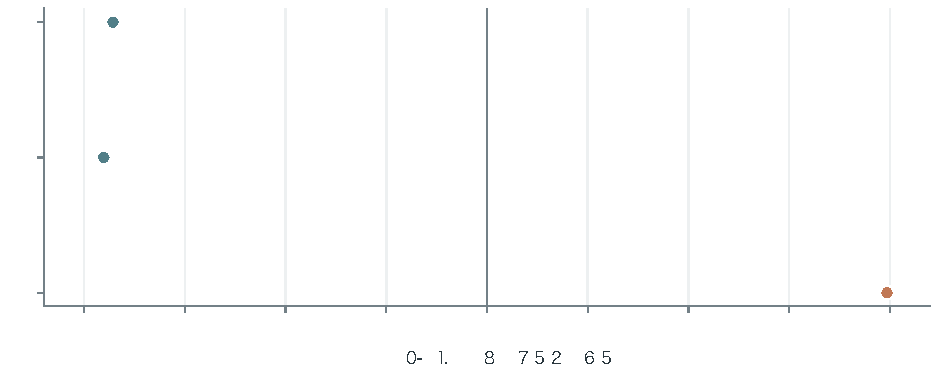
\includegraphics[width=0.82\linewidth]{figures/q2-scaling-law/FigS01_B8_quality_direction.pdf}
\caption{B6、B7、B8 在固定 $(N,D)$ 组内的质量--Loss Spearman 相关中位数}
\label{fig:q2-b8}
\end{figure}

\begin{figure}[htbp]
\centering
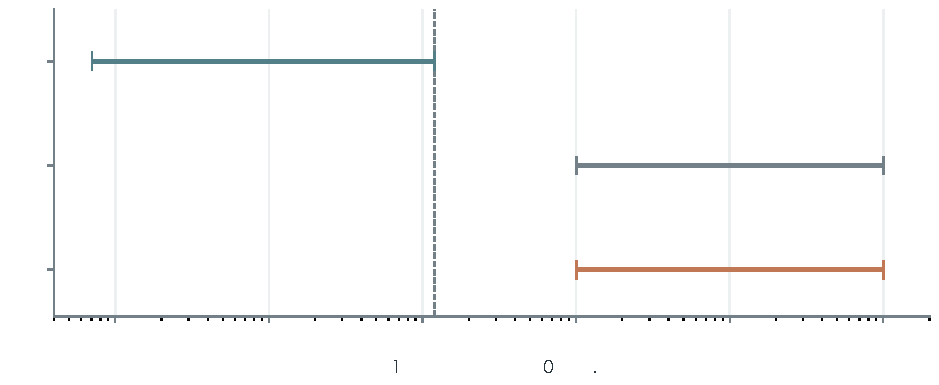
\includegraphics[width=0.82\linewidth]{figures/q2-scaling-law/FigS02_large_model_range.pdf}
\caption{B1 主拟合、B9 元数据与 B10 估算材料的参数范围}
\label{fig:q2-range}
\end{figure}

现阶段可以回答：B1 内部幂律优于对数线性原型；半合成 B6/B7 中质量项有局部增量；A 侧同规模配比有预测信息；条件模型的边际效用递减、可行替代范围和结构性零交互可由公式及数值核查。尚不能给出整个 $N,D,Q_A,\boldsymbol p$ 模型的独立联合误差、真实质量干预收益、领域互补强度或无条件的大模型外推准确率。后续须获取共同观测四类输入以及对应的Loss实验数据，进行建模，拟合和测试等论题探讨。目前式~\eqref{eq:q2-joint} 依据当前条件推导出，作为资源配置情景分析的条件目标函数。
